\documentclass[a4paper]{jarticle}
% \documentclass[a5j]{jsarticle}


\usepackage{amsfonts,latexsym}
\usepackage{ulem}
\usepackage{fancybox}
\usepackage[dvipdfmx]{graphicx}
\usepackage[deluxe]{otf}
\usepackage[margin=20truemm]{geometry}

\usepackage{pifont}
\usepackage{amsmath}

\DeclareFontShape{JT1}{hmc}{b}{n}{<->ssub*hmc/bx/n}{}
\DeclareFontShape{JY1}{hmc}{b}{n}{<->ssub*hmc/bx/n}{}

% ==============================================
% page format
%  textwidth  = paperwidth(210mm) -oddsidemargin(13mm) -evensidemargin(13mm)
%  textheight = paperheight(297mm) -topmargin(20mm-header分) -bottommargin(18mm)
% ==============================================
  \setlength{\paperwidth}{210mm}
  \setlength{\textwidth}{\paperwidth}
  \addtolength{\textwidth}{-13mm} % oddside margin
  \addtolength{\textwidth}{-13mm} % evenside margin
  \setlength{\oddsidemargin}{-1in}
  \addtolength{\oddsidemargin}{13mm} %%%% ここで左右を調節
%
  \setlength{\paperheight}{297mm}
  \setlength{\textheight}{\paperheight}
  \addtolength{\textheight}{-10mm} % 文章領域の高さの調整
  \addtolength{\textheight}{-23truemm}  
  \setlength{\topmargin}{-17mm}    % ここで上下位置を調節
%
  \setlength{\headheight}{0in}
  \setlength{\headsep}{0in}
  \setlength{\columnsep}{10mm}

%   \pagestyle{plain}
  \pagestyle{empty}

% ========================================
% タイトルの書式設定(開始)
  \makeatletter
   \def\@maketitle{%
   \newpage\null
   \vskip 2em%
   \begin{center}%
   \let\footnote\thanks
     \vspace{-15mm}
     {\LARGE \@title \par}%
     \vskip 1.5em%
   \end{center}
   \begin{flushright}
     {\large
       \lineskip .5em%
       \begin{tabular}[t]{c}%
         \@author
       \end{tabular}\par}%
     \vskip 1em%
%      {\large \@date}%
   \end{flushright}%
   \par\vskip 1.5em}
   \vspace{10mm}
   \renewcommand{\section}{\@startsection{section}{1}{\z@}%
   {1.5\Cvs \@plus.5\Cvs \@minus.2\Cvs}%
   {.5\Cvs \@plus.3\Cvs}%\and
   {\reset@font\large\bfseries}}   %section見出しの文字サイズをlargeに変更
   
   % 参考文献の書式設定
   \renewenvironment{thebibliography}[1]
{\section*{\refname\@mkboth{\refname}{\refname}}%
  \list{\@biblabel{\@arabic\c@enumiv}}%
       {\settowidth\labelwidth{\@biblabel{#1}}%
        \leftmargin\labelwidth
        \advance\leftmargin\labelsep
%  \setlength\itemsep{-0.5zh}%←ここの数値を調整(行間のつまり具合)
 \setlength\baselineskip{12pt}%←ここの数値を調整(追加)(文字の大きさ)
        \@openbib@code
        \usecounter{enumiv}%
        \let\p@enumiv\@empty
        \renewcommand\theenumiv{\@arabic\c@enumiv}}%
  \sloppy
  \clubpenalty4000
  \@clubpenalty\clubpenalty
  \widowpenalty4000%
  \sfcode`\.\@m}
 {\def\@noitemerr
   {\@latex@warning{Empty `thebibliography' environment}}%
  \endlist}
  \makeatother
% タイトルの書式設定(終わり)
% ========================================


%ここから下を変更する
  \title{CtoC Bike Shareにおけるマッチングモデルの提案と実装と検証と}
  \author{風折晃輝}
  \date{\today}


\fontsize{10.5mm}{0pt}

\begin{document}

\twocolumn[
 \begin{center}
  {\Large 第3回KP}\\
  \rule{\textwidth}{1mm}
 \end{center}
 \maketitle
  \thispagestyle{empty}
]


% 本文 =====================================

%\noindent

% section 1 ----
\section{はじめに}
\vspace{-3mm}
\par 欧米やアジアを中心に,自転車を好きなタイミングで好きな期間利用することができるシェアサイクルサービスが世界的に普及している.しかし,個人が所有している自転車はシェアリングの対象になっていない.あらゆる地域に散在している個人所有の自転車をモビリティのリソースとして有効活用できれば,交通手段の多様化と効率化が促進され,環境負荷の軽減や都市交通の改善にも寄与できるのではないだろうか.そこで,個人所有の自転車を個人間で効率的にシェアリングするため,数理最適化ベースで自転車の割り当てモデルを構築する.

% \vspace{-3mm}

% section 2 ----
\section{数理最適化ベースの自転車割り当てモデル}
\vspace{-3mm}
\par 個人所有の自転車をシェアリングの対象とし,ユーザ体験の観点からドックレスで乗り捨て可能なシステムを前提とする.なお,乗り捨てによる自転車の不法駐輪等の法的な課題に関してはここでは考慮せず,あくまで自転車の割り当て問題として切り分けてモデリングする.
\par ユーザリクエストの集合を$J$,シェアリングされる自転車の集合を$B$,ユーザ$j(j \in J)$に自転車$b(b \in B)$が割り当てられたか否かの二値変数行列を$x_{b,j}$,割り当て移動後の距離行列を$d_{b,j}$とする.目的関数は(1)式のように定義し,集合$J$の全てのユーザが移動した後の自転車の散らばりを最小化し,より多くのユーザに自転車を割り当てることを目指す.ただし,$\alpha$は$x_{b,j}$に対する重みである.

\vspace{-8mm}

\begin{flushright}
\begin{equation}
\min \left( \sum_{b}\sum_{j}d_{b,j}x_{b,j} - \alpha\sum_{b}\sum_{j}x_{b,j} \right) \tag{1}
\end{equation}
\end{flushright}

% \vspace{-3mm}

% section 3 ----
\section{NYCタクシーデータを用いたシミュレート}
\vspace{-3mm}
\par 構築したモデルを評価・検証するため,C2Cドックレスシェアサイクルの需要に最も親和性が高いと考えられるタクシーの利用データを用いてシミュレーションを行う.シミュレーションに用いるタクシーデータはニューヨーク市(NYC)のタクシー・リムジン委員会(TLC)から提供されている2023年1月のNYCのイエロータクシーのトリップデータを使用することとする.可能な限りドックレスであるシステムの実現を目指すため,ユーザからのリクエストは1分ごとの集合$J$として集約し,(1)式にて定義したモデルに入力し,その他定式化した制約条件のもと割り当て処理を実行する.また,自転車はNYCの主要な約250ポイントのうち,ランダムに10ポイント選択して配置する.
\par 評価方法については,結果として出力される二値変数行列$x_{b,j}$や自転車のステータスを保持する$B$などを元に行う.

% \vspace{-3mm}

% section 4 ----
\section{結果と考察}
\vspace{-3mm}
\par 2023年1月1日の24時間のトリップデータを連続的にモデルに入力し,結果的にユーザからのリクエストに対して自転車を割り当てることができた割合と,その際に既に利用中の自転車がどれくらいの割合であったかを示す占有率,サービス提供後に自転車を再配置するためのリバランスコストを算出した.特にKPIとして設定しているリバランスコストに対して,別の割り当てモデルを構築し比較すると図\ref{fig:resultFig}のような結果となった.リバランスコストは本モデルが最も優位な値で推移している

\begin{figure}[b]
  \centering
  \vspace{-5mm}  % 図の前のスペースを減らす
  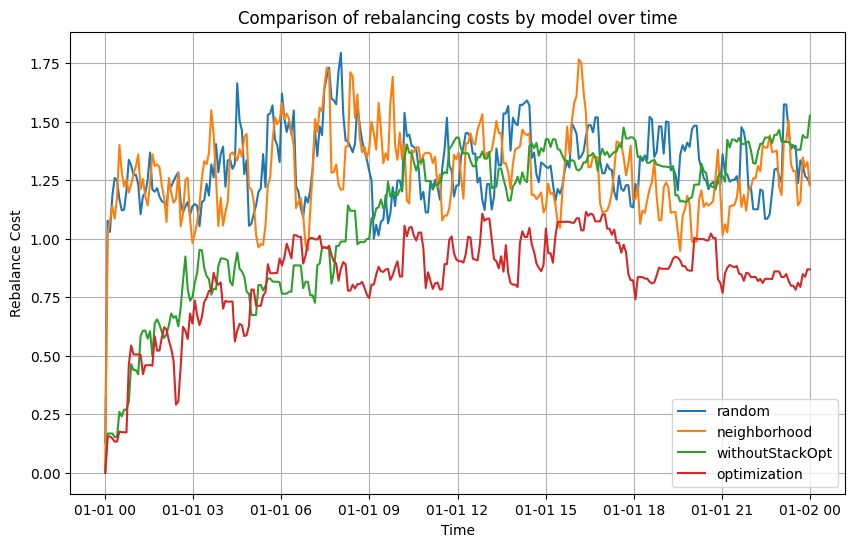
\includegraphics[scale=0.4]
  {figures/compariso-rebalancing-costs.png}
  \vspace{-5mm}
  \caption{モデル毎の再配置コストの比較}
  \label{fig:resultFig}
  \vspace{-5mm}  % 図の後のスペースを減らす
\end{figure}


% \vspace{-3mm}

% section 5 ----
\section{まとめと今後の方針}
\vspace{-3mm}
個人間シェアリングシステムに実装するにあたって,より制約条件をスケールしていく必要がある.例えば,「分散を最小化する」かつ「システムの収益を最大化する」という最小化指標と最大化指標の複数指標で議論しなければならない.ただ,分散を最小化することを最優先として考え,より最適なモデルを構築することを目指す.

% \vspace{-3mm}

% section 6 ----
\section{プレゼンテーションバッファ}
時間が余れば,本研究にてAPIを構築する上で出会い,感動したテストツール・ライブラリのschemathesisについて,何ができてどうすごいのかについて紹介する.

% \bibliographystyle{junsrt}
% \bibliography{sannkou.bib}
% ==============================================
% 原稿はここまで
% ==============================================
\end{document}
